\chapter{Results and Discussion}
\label{chap:results}

\section{Study Overview}
The study evaluated prior choice, predictive performance and posterior interpretation within one comparative framework. Normal, horseshoe and continuous spike-and-slab priors shared a Bayesian piecewise-exponential proportional-hazards likelihood, predictor representation and validation partitions. Cox proportional-hazards regression (CoxPH), random survival forest (RSF) and DeepSurv provided statistical, ensemble and neural comparators.

Five repeats of five-fold outer cross-validation yielded \ConfirmatoryPlanned{} model--fold outcomes across GBSG2, WHAS500 and METABRIC. Of these, \ConfirmatoryComplete{} supplied accepted predictions. All comparators, Normal-prior models and continuous spike-and-slab models completed 25 evaluations per cohort. The horseshoe arm supplied seven accepted evaluations in GBSG2, 25 in WHAS500 and 23 in METABRIC. The \ConfirmatoryFailed{} remaining outcomes did not meet the sampling criteria. Coverage is reported alongside each result, allowing predictive estimates and computational reliability to be interpreted together.

Preprocessing and model selection used training data within each validation partition. Integrated Brier score (IBS) measured probability prediction error, Uno's concordance measured discrimination under censoring, and time-dependent AUC and calibration described further aspects of prediction. Within-cohort paired contrasts used identical validation subjects and training-defined evaluation times. The uncertainty calculation accounts approximately for the overlapping training samples in repeated cross-validation, as described in Chapter~\ref{chap:methods}. Fold standard deviations describe variation across these repeated evaluations.

\section{Cohort Characteristics and Survival Patterns}
\label{sec:cohort-results}
The three cohorts represent distinct clinical settings. GBSG2 contains 686 patients and 299 events on its distributed recurrence-free-survival endpoint. WHAS500 contains 500 patients and 215 deaths following admission for acute myocardial infarction. METABRIC contains 1,980 eligible patients and 1,144 deaths on its overall-survival endpoint. Table~\ref{tab:gen-cohorts} summarises these analysis populations.

% Generated from hash-verified saved evidence. Do not edit by hand.
\begin{table}[htbp]
\centering
\caption{Eligible analysis cohorts and observed outcomes.}
\label{tab:gen-cohorts}
\small
\setlength{\tabcolsep}{3pt}
\begin{adjustbox}{max width=\textwidth}
\begin{tabular}{lrrrll}
\toprule
Cohort & $n$ & Events & Censored (\%) & Endpoint & Time unit \\
\midrule
GBSG2 & 686 & 299 & 387 (56.4) & Recurrence-free survival & days \\
WHAS500 & 500 & 215 & 285 (57.0) & All-cause mortality & days \\
METABRIC & 1,980 & 1,144 & 836 (42.2) & Overall survival & months \\
\bottomrule
\end{tabular}
\end{adjustbox}
\par\smallskip
\begin{minipage}{\textwidth}\footnotesize METABRIC eligibility includes positive observed follow-up. Endpoints and time units are cohort-specific.\end{minipage}
\end{table}


GBSG2 and WHAS500 record follow-up in days; METABRIC records overall survival in months. Censoring proportions are 56.4\%, 57.0\% and 42.2\%, respectively. Each cohort was analysed separately, with matched model comparisons within the cohort. This design allows the empirical behaviour of the priors to be examined across different event patterns, clinical predictors and amounts of information.

The primary predictors describe the clinical information specified for each setting. GBSG2 includes tumour, receptor, lymph-node, patient and trial-treatment variables. WHAS500 uses the admission-time predictor specification. METABRIC uses diagnosis and pathology variables, with controlled representation of Nottingham Prognostic Index and its components. Training-fold imputation, encoding and scaling preserved the separation between model development and evaluation. Appendix~\ref{app:data} provides the predictor definitions and missingness summaries.

Figure~\ref{fig:km} shows the Kaplan--Meier survival estimates with their native time scales. These curves describe each cohort's event experience under right censoring. The intervals widen as fewer patients remain at risk later in follow-up. Observed follow-up summaries and censoring-adjusted survival medians are given in Appendix~\ref{app:exploratory}.

\begin{figure}[tbp]
\centering
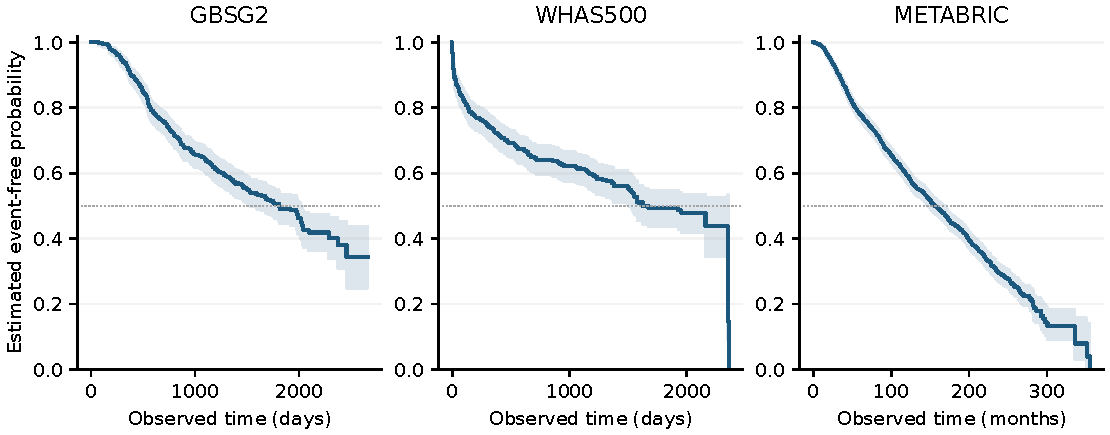
\includegraphics[width=\linewidth,height=0.72\textheight,keepaspectratio]{generated/figure_kaplan_meier.pdf}
\caption[Kaplan--Meier estimates by cohort.]{Kaplan--Meier estimates for the three clinical cohorts, with pointwise confidence intervals. Each panel uses its cohort's endpoint and native follow-up unit.}
\label{fig:km}
\end{figure}

\section{Predictive Performance and Prior Choice}
\label{sec:predictive-results}
\subsection{Performance Across Model Families}
Table~\ref{tab:gen-predictive-metrics} presents the mean and sample standard deviation of the evaluation metrics across accepted outer folds. Higher concordance and AUC indicate better discrimination, while lower IBS indicates lower probability prediction error. The table also reports the number of accepted evaluations for each cohort and model.

% Generated from hash-verified saved evidence. Do not edit by hand.
\begin{table}[htbp]
\centering
\caption{Repeated-validation predictive performance by cohort and model.}
\label{tab:gen-predictive-metrics}
\small
\setlength{\tabcolsep}{3pt}
\begin{adjustbox}{max width=\textwidth}
\begin{tabular}{llrrrrr}
\toprule
Cohort & Model & $n$ & Harrell $C$ & Uno $C$ & IBS & Mean AUC \\
\midrule
GBSG2 & CoxPH & 25/25 & 0.6752 (0.0243) & 0.6792 (0.0262) & 0.1673 (0.0058) & 0.7331 (0.0328) \\
GBSG2 & RSF & 25/25 & 0.6915 (0.0207) & 0.6942 (0.0233) & 0.1624 (0.0071) & 0.7513 (0.0303) \\
GBSG2 & DeepSurv & 25/25 & 0.6768 (0.0287) & 0.6840 (0.0315) & 0.1653 (0.0083) & 0.7365 (0.0375) \\
GBSG2 & Normal & 25/25 & 0.6751 (0.0245) & 0.6790 (0.0265) & 0.1672 (0.0056) & 0.7334 (0.0332) \\
GBSG2 & Horseshoe & 7/25 & 0.6800 (0.0202) & 0.6879 (0.0271) & 0.1678 (0.0058) & 0.7530 (0.0310) \\
GBSG2 & Spike-and-slab & 25/25 & 0.6752 (0.0246) & 0.6792 (0.0266) & 0.1672 (0.0055) & 0.7337 (0.0335) \\
WHAS500 & CoxPH & 25/25 & 0.7500 (0.0258) & 0.7501 (0.0245) & 0.1525 (0.0114) & 0.7693 (0.0363) \\
WHAS500 & RSF & 25/25 & 0.7461 (0.0345) & 0.7449 (0.0328) & 0.1551 (0.0108) & 0.7645 (0.0479) \\
WHAS500 & DeepSurv & 25/25 & 0.7406 (0.0300) & 0.7430 (0.0309) & 0.1557 (0.0110) & 0.7614 (0.0432) \\
WHAS500 & Normal & 25/25 & 0.7502 (0.0262) & 0.7501 (0.0254) & 0.1524 (0.0112) & 0.7697 (0.0369) \\
WHAS500 & Horseshoe & 25/25 & 0.7507 (0.0288) & 0.7506 (0.0276) & 0.1521 (0.0109) & 0.7691 (0.0389) \\
WHAS500 & Spike-and-slab & 25/25 & 0.7504 (0.0263) & 0.7503 (0.0256) & 0.1523 (0.0111) & 0.7699 (0.0370) \\
METABRIC & CoxPH & 25/25 & 0.6573 (0.0153) & 0.6568 (0.0172) & 0.1885 (0.0047) & 0.6883 (0.0203) \\
METABRIC & RSF & 25/25 & 0.6774 (0.0154) & 0.6779 (0.0162) & 0.1806 (0.0044) & 0.7207 (0.0179) \\
METABRIC & DeepSurv & 25/25 & 0.6682 (0.0158) & 0.6680 (0.0165) & 0.1857 (0.0048) & 0.7043 (0.0208) \\
METABRIC & Normal & 25/25 & 0.6570 (0.0152) & 0.6565 (0.0169) & 0.1886 (0.0045) & 0.6875 (0.0202) \\
METABRIC & Horseshoe & 23/25 & 0.6565 (0.0143) & 0.6559 (0.0160) & 0.1888 (0.0040) & 0.6858 (0.0197) \\
METABRIC & Spike-and-slab & 25/25 & 0.6570 (0.0151) & 0.6564 (0.0169) & 0.1886 (0.0045) & 0.6874 (0.0201) \\
\bottomrule
\end{tabular}
\end{adjustbox}
\par\smallskip
\begin{minipage}{\textwidth}\footnotesize Entries are unweighted means (sample SD) across accepted outer folds from five repeats of five-fold validation. The $n$ column gives accepted/total evaluations. Horseshoe summaries use seven GBSG2 and 23 METABRIC fits. Paired inference is reported separately. Higher concordance/AUC and lower IBS indicate better prediction.\end{minipage}
\end{table}


In GBSG2, RSF had mean IBS 0.1624, followed by DeepSurv at 0.1653. CoxPH, Normal and continuous spike-and-slab gave values close to 0.1672--0.1673. RSF also had the highest mean Uno concordance among the models with 25 accepted evaluations, at 0.6942. Thus the forest's descriptive advantage appeared in both probability error and discrimination in this cohort.

WHAS500 showed a different pattern. The complete Bayesian arms and CoxPH had mean IBS values between 0.1521 and 0.1525, compared with 0.1551 for RSF and 0.1557 for DeepSurv. Uno concordance was close to 0.750 for CoxPH and the Bayesian models. These results show that the simpler linear risk structures represented the selected WHAS500 predictors effectively within this validation design.

METABRIC had a clearer separation between model families. RSF had mean IBS 0.1806 and Uno concordance 0.6779; DeepSurv had IBS 0.1857 and Uno concordance 0.6680. The corresponding Normal-prior values were 0.1886 and 0.6565. CoxPH and continuous spike-and-slab were close to Normal on both metrics. The horseshoe summaries in GBSG2 and METABRIC describe their accepted subsets, with seven and 23 folds contributing to the respective means.

\begin{figure}[tbp]
\centering
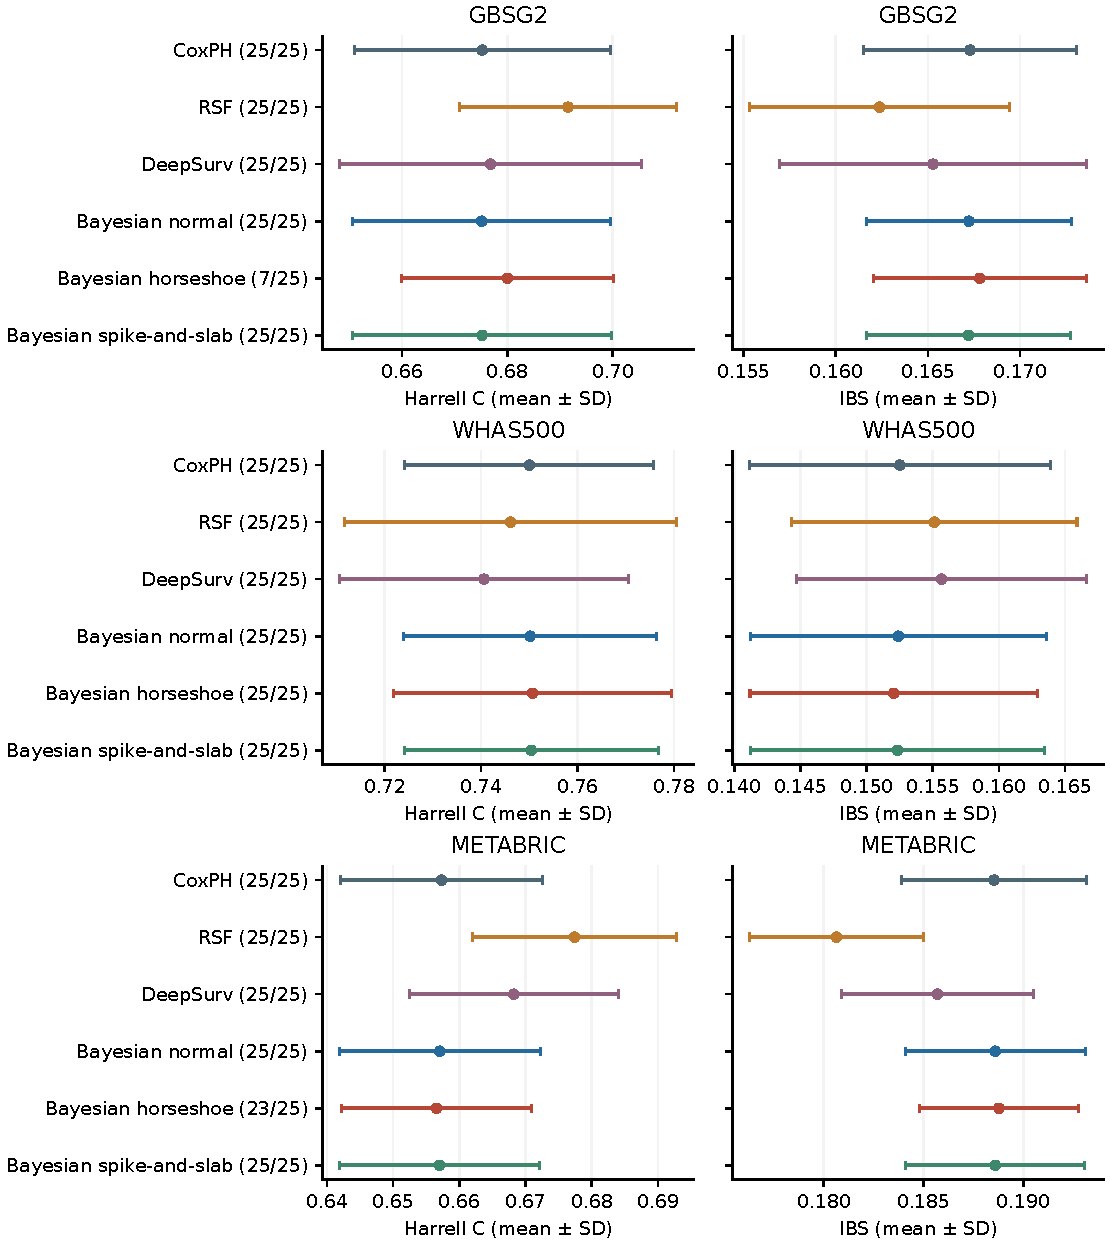
\includegraphics[width=\linewidth,height=0.75\textheight,keepaspectratio]{generated/figure_predictive_metrics.pdf}
\caption[Prediction error and discrimination by model.]{Probability prediction error and discrimination across the three cohorts. Summaries use accepted outer-fold evaluations; fold counts identify the contribution to each estimate.}
\label{fig:predictive-overview}
\end{figure}

\subsection{Paired Comparisons with CoxPH, RSF and DeepSurv}
The paired comparator estimates provide uncertainty around these descriptive differences. Table~\ref{tab:report-secondary} uses Normal as a common reference because it has complete original coverage in every cohort. Each difference is IBS(Normal) minus IBS(comparator), so a positive value favours the comparator. These are secondary estimates with repeated-validation intervals.

\begin{table}[htbp]
\centering
\small
\caption{Secondary paired IBS contrasts for the Normal-prior reference.}
\label{tab:report-secondary}
\begin{tabular}{@{}llr@{}}
\toprule
Cohort & Comparator & Normal minus comparator [95\% interval]\\
\midrule
GBSG2 & CoxPH & -0.000065 [-0.000414, +0.000284]\\
GBSG2 & RSF & +0.004848 [-0.002582, +0.012277]\\
GBSG2 & DeepSurv & +0.001946 [-0.005759, +0.009652]\\
WHAS500 & CoxPH & -0.000116 [-0.001077, +0.000846]\\
WHAS500 & RSF & -0.002719 [-0.011879, +0.006442]\\
WHAS500 & DeepSurv & -0.003269 [-0.011456, +0.004918]\\
METABRIC & CoxPH & +0.000054 [-0.000241, +0.000349]\\
METABRIC & RSF & +0.007956 [+0.004531, +0.011381]\\
METABRIC & DeepSurv & +0.002893 [+0.000707, +0.005079]\\
\bottomrule
\end{tabular}
\par\smallskip
\begin{minipage}{\textwidth}\footnotesize All rows use 25 matched outer evaluations. Negative differences favour Normal, the common reference with complete coverage in every cohort. Intervals use the repeated-validation correction. These are secondary estimates.\end{minipage}
\end{table}


Normal and CoxPH had closely aligned prediction error. Their mean paired differences were -0.000065 in GBSG2, -0.000116 in WHAS500 and +0.000054 in METABRIC. Each interval included zero. This comparison is informative because both use a linear proportional-hazards risk function, while differing in likelihood and estimation. The Bayesian model supplied posterior coefficient distributions while retaining closely aligned average IBS for these predictor sets.

The Normal minus RSF difference was +0.004848 in GBSG2, with a corrected 95\% interval of [-0.002582, +0.012277]. In WHAS500 it was -0.002719 [-0.011879, +0.006442]. METABRIC gave +0.007956 [+0.004531, +0.011381], the clearest separation among these comparisons. Normal minus DeepSurv was also positive in METABRIC, at +0.002893 [+0.000707, +0.005079], while its GBSG2 and WHAS500 intervals included zero.

These cohort-specific patterns agree with the broader survival-benchmark literature, in which model performance varies with dataset and evaluation design \cite{ravi33,ravi37,ravi52,ravi70}. RSF and DeepSurv can represent nonlinear risk relationships, whereas the Bayesian arms and CoxPH use linear risk scores. Their fitted predictions also reflect the chosen tuning, baseline-hazard treatment and predictor representation. The paired results quantify the overall differences between the evaluated implementations.

\subsection{Primary Comparisons Between Coefficient Priors}
The primary comparisons isolate coefficient-prior choice within the common Bayesian model. Table~\ref{tab:gen-primary-contrasts} reports IBS($A$) minus IBS($B$), with negative values favouring $A$. The three pairwise prior contrasts in each cohort form the nine-comparison primary family.

% Generated from hash-verified saved evidence. Do not edit by hand.
\begin{table}[htbp]
\centering
\caption{Prespecified paired IBS contrasts between Bayesian priors.}
\label{tab:gen-primary-contrasts}
\small
\setlength{\tabcolsep}{3pt}
\begin{adjustbox}{max width=\textwidth}
\begin{tabular}{llrrrr}
\toprule
Cohort & Contrast ($A-B$) & Pairs & $\Delta$IBS & Nominal 95\% interval & $p$ \\
\midrule
GBSG2 & Normal - Horseshoe & 7/25 & -- & -- & -- \\
GBSG2 & Normal - Spike-and-slab & 25/25 & +0.000025 & [-0.000103, +0.000153] & 0.693 \\
GBSG2 & Horseshoe - Spike-and-slab & 7/25 & -- & -- & -- \\
WHAS500 & Normal - Horseshoe & 25/25 & +0.000344 & [-0.001706, +0.002395] & 0.732 \\
WHAS500 & Normal - Spike-and-slab & 25/25 & +0.000061 & [-0.000120, +0.000242] & 0.493 \\
WHAS500 & Horseshoe - Spike-and-slab & 25/25 & -0.000284 & [-0.002174, +0.001607] & 0.760 \\
METABRIC & Normal - Horseshoe & 23/25 & -- & -- & -- \\
METABRIC & Normal - Spike-and-slab & 25/25 & -0.000008 & [-0.000087, +0.000071] & 0.833 \\
METABRIC & Horseshoe - Spike-and-slab & 23/25 & -- & -- & -- \\
\bottomrule
\end{tabular}
\end{adjustbox}
\par\smallskip
\begin{minipage}{\textwidth}\footnotesize Differences are IBS($A$) minus IBS($B$); negative values favour $A$. Intervals and two-sided tests use the Nadeau--Bengio repeated-validation correction. Inference requires all 25 matched folds; four contrasts have partial coverage. Holm bounds for the nine-contrast family appear in Table~\ref{tab:gen-holm-bounds}.\end{minipage}
\end{table}


Normal and continuous spike-and-slab differed by +0.000025 in GBSG2, +0.000061 in WHAS500 and -0.000008 in METABRIC. Their corrected 95\% intervals all included zero. These estimates show that the two priors produced closely aligned probability predictions across the three clinical settings.

WHAS500 supplied complete pairing for all three prior contrasts. Normal minus horseshoe was +0.000344 [-0.001706, +0.002395], and horseshoe minus continuous spike-and-slab was -0.000284 [-0.002174, +0.001607]. Their point estimates were small relative to the interval widths. Taken with the complete Normal versus continuous spike-and-slab comparisons, five primary contrasts had all 25 matched evaluations. The other four involved horseshoe in GBSG2 or METABRIC and are reported with their available fold counts rather than a complete-fold effect estimate.

\begin{figure}[tbp]
\centering
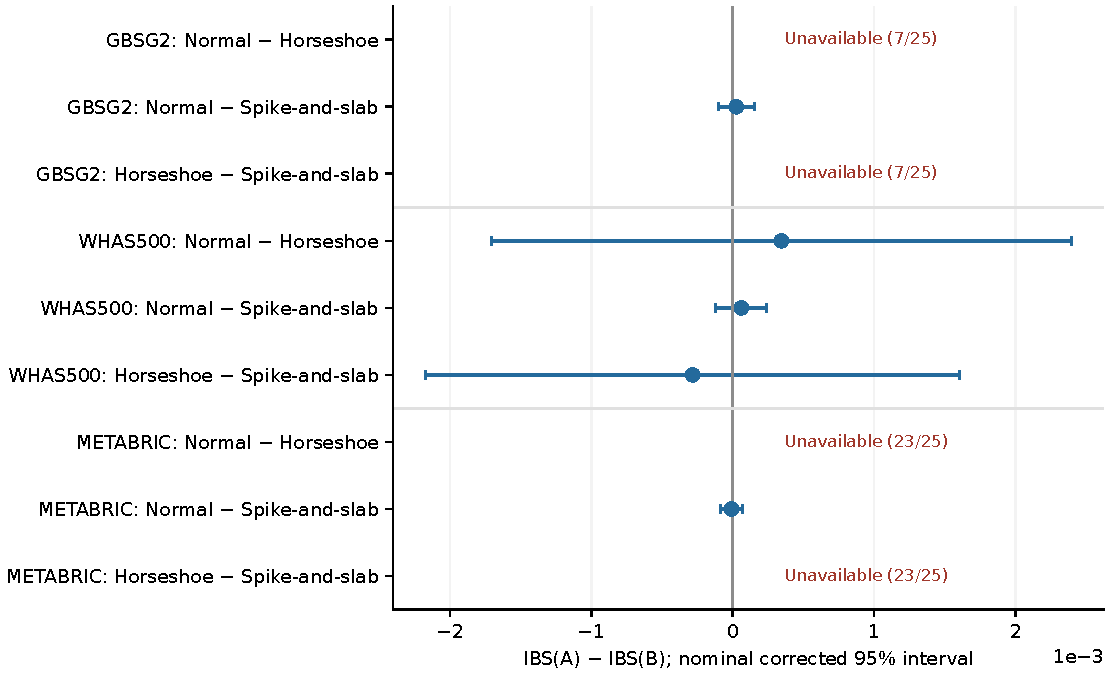
\includegraphics[width=\linewidth,height=0.7\textheight,keepaspectratio]{generated/figure_primary_contrasts.pdf}
\caption[Paired primary IBS contrasts.]{Paired primary IBS differences with nominal 95\% repeated-validation intervals. Contrasts require 25 accepted matched evaluations; coverage is shown for the other comparisons.}
\label{fig:primary-contrasts}
\end{figure}

The primary evidence therefore places the predictive effects of Normal and continuous spike-and-slab close to zero within these clinical predictor sets. The intervals quantify uncertainty around their differences; they are not equivalence intervals. The complete WHAS500 comparisons add a corresponding estimate for horseshoe. The post-hoc analysis in Section~\ref{sec:posthoc-results} examines that arm under a different sampler setting.

\section{Calibration of Survival Predictions}
\label{sec:calibration-results}
Calibration examines agreement between predicted event probabilities and observed outcomes after accounting for censoring. It complements discrimination and IBS by describing both the overall level and spread of the predictions \cite{ravi26,ravi60,ravi88}. Table~\ref{tab:gen-calibration} summarises the middle evaluation horizon, defined from the median training-event time in each fold.

% Generated from hash-verified saved evidence. Do not edit by hand.
\begin{table}[htbp]
\centering
\caption{Calibration estimates at each fold's middle prespecified horizon.}
\label{tab:gen-calibration}
\small
\setlength{\tabcolsep}{3pt}
\begin{adjustbox}{max width=\textwidth}
\begin{tabular}{llrrrr}
\toprule
Cohort & Model & $n$ & Calibration-in-large & Intercept & Slope \\
\midrule
GBSG2 & CoxPH & 25 & -0.037 (0.129) & 0.216 (0.553) & 1.186 (0.417) \\
GBSG2 & RSF & 25 & -0.002 (0.082) & 0.121 (0.327) & 1.119 (0.311) \\
GBSG2 & DeepSurv & 25 & -0.052 (0.110) & 0.005 (0.384) & 1.040 (0.292) \\
GBSG2 & Normal & 25 & -0.003 (0.101) & 0.309 (0.548) & 1.244 (0.409) \\
GBSG2 & Horseshoe & 7 & -0.038 (0.101) & 0.191 (0.663) & 1.175 (0.516) \\
GBSG2 & Spike-and-slab & 25 & -0.003 (0.100) & 0.317 (0.551) & 1.250 (0.411) \\
WHAS500 & CoxPH & 25 & -0.005 (0.132) & -0.087 (0.309) & 0.912 (0.234) \\
WHAS500 & RSF & 25 & 0.004 (0.095) & 0.114 (0.538) & 1.097 (0.448) \\
WHAS500 & DeepSurv & 25 & -0.010 (0.114) & -0.064 (0.360) & 0.943 (0.295) \\
WHAS500 & Normal & 25 & 0.010 (0.125) & -0.038 (0.316) & 0.947 (0.241) \\
WHAS500 & Horseshoe & 25 & 0.006 (0.114) & 0.028 (0.331) & 1.017 (0.264) \\
WHAS500 & Spike-and-slab & 25 & 0.010 (0.124) & -0.034 (0.316) & 0.952 (0.242) \\
METABRIC & CoxPH & 25 & -0.015 (0.041) & -0.098 (0.160) & 0.905 (0.161) \\
METABRIC & RSF & 25 & 0.005 (0.039) & 0.129 (0.228) & 1.145 (0.241) \\
METABRIC & DeepSurv & 25 & -0.024 (0.041) & -0.049 (0.185) & 0.970 (0.202) \\
METABRIC & Normal & 25 & 0.002 (0.040) & -0.066 (0.167) & 0.924 (0.167) \\
METABRIC & Horseshoe & 23 & 0.003 (0.039) & -0.039 (0.178) & 0.954 (0.178) \\
METABRIC & Spike-and-slab & 25 & 0.002 (0.039) & -0.065 (0.168) & 0.926 (0.167) \\
\bottomrule
\end{tabular}
\end{adjustbox}
\par\smallskip
\begin{minipage}{\textwidth}\footnotesize Entries are accepted-fold means (sample SD) at the training-event median horizon. Ideal calibration-in-the-large and intercept are zero; ideal slope is one. Each fold defines its horizon from its own training data.\end{minipage}
\end{table}


For Normal and continuous spike-and-slab in GBSG2, mean calibration slopes were 1.244 and 1.250, with fold standard deviations of 0.409 and 0.411. Under the complementary-log-log calibration model, slopes above one indicate that the predictions have less spread than the fitted observed relationship. WHAS500 slopes were closer to one, at 0.947 and 0.952, while METABRIC gave 0.924 and 0.926. Slopes below one indicate the reverse pattern of spread. Figure~\ref{fig:calibration-summary} displays this variation alongside calibration intercepts.

\begin{figure}[p]
\centering
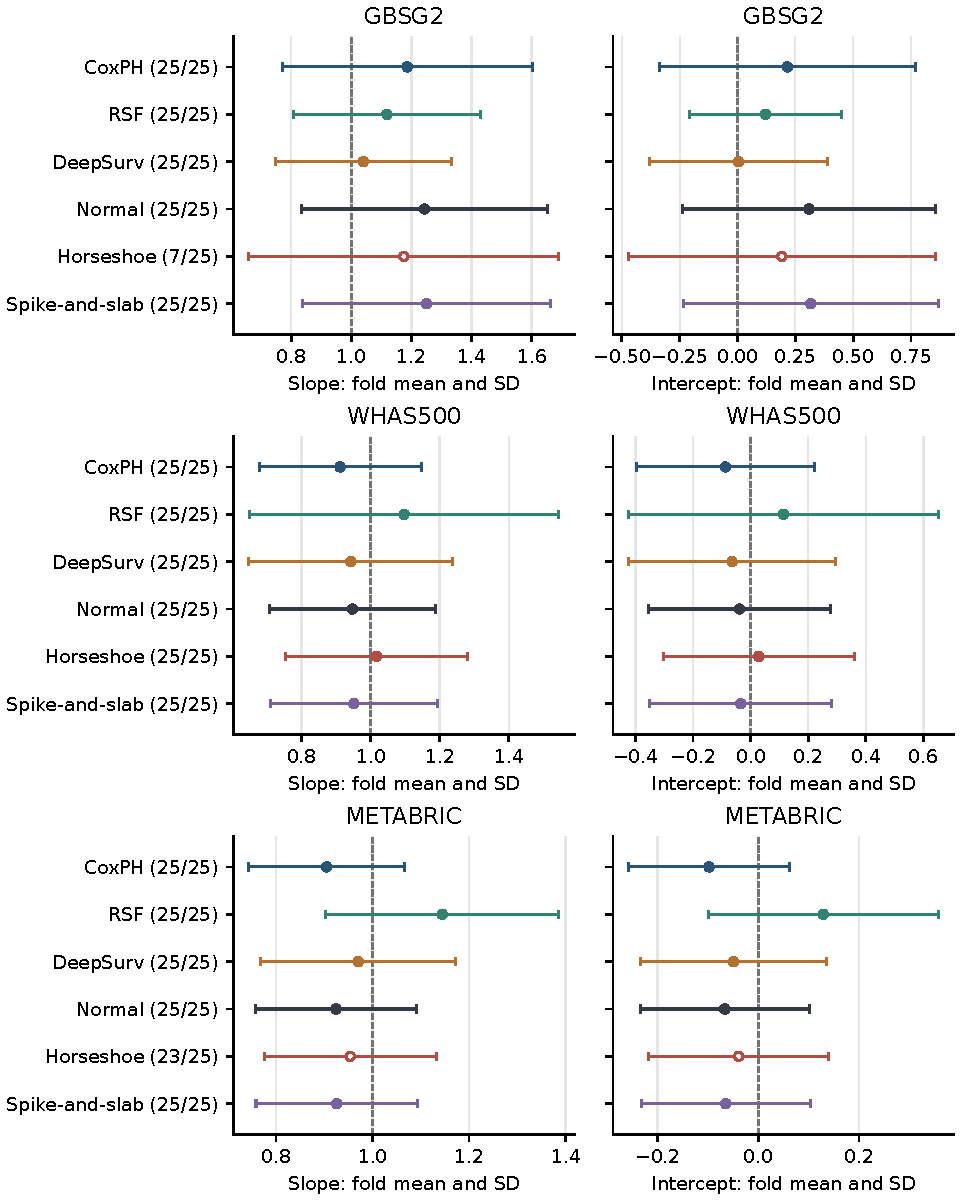
\includegraphics[width=\linewidth,height=0.79\textheight,keepaspectratio]{report_summaries/figure_calibration_summary.pdf}
\caption[Calibration slopes and intercepts.]{Calibration slopes and intercepts at the middle training-defined horizon. Points are fold means, bars are one sample standard deviation, and reference lines indicate slope one and intercept zero. Open points identify partial horseshoe coverage.}
\label{fig:calibration-summary}
\end{figure}

Calibration-in-the-large, estimated as a complementary-log-log intercept with slope fixed at one, was close to zero on average for Normal: -0.003 in GBSG2, +0.010 in WHAS500 and +0.002 in METABRIC. Continuous spike-and-slab gave the same values to three decimal places. This fixed-slope intercept describes a common shift on the calibration link scale, while the freely estimated slope describes the spread of the predictions.

The jointly estimated calibration intercepts also differed between cohorts. Normal had mean intercept 0.309 in GBSG2, -0.038 in WHAS500 and -0.066 in METABRIC, with fold standard deviations 0.548, 0.316 and 0.167. These intercepts belong to the fitted slope--intercept relationship, whereas calibration-in-the-large uses the fixed-slope model. Together, the summaries show how calibration distinguishes models whose mean IBS values are close. All three training-defined horizons are reported in Appendix~\ref{app:predictive}.

\section{Posterior Interpretation and Explanation Agreement}
\label{sec:explanation-results}
\subsection{Interpreting Coefficients and Hazard Ratios}
Posterior distributions connect the prediction model to interpretable associations with clinical predictors. Table~\ref{tab:gen-posterior-examples} gives examples from the first outer Normal-prior fit, using a fixed cohort, fold and prior rule. It reports posterior coefficient means, mean hazard ratios, 95\% credible intervals and probabilities that the coefficient is positive.

% Generated from hash-verified saved evidence. Do not edit by hand.
\begin{table}[htbp]
\centering
\caption{Illustrative posterior summaries from the first outer normal-prior fit.}
\label{tab:gen-posterior-examples}
\small
\setlength{\tabcolsep}{3pt}
\begin{adjustbox}{max width=\textwidth}
\begin{tabular}{llrrrr}
\toprule
Cohort & Feature & $E[\beta]$ & $E[\mathrm{HR}]$ & HR 95\% credible interval & $P(\beta>0)$ \\
\midrule
GBSG2 & Positive lymph nodes & 0.263 & 1.303 & [1.183, 1.420] & 1.000 \\
GBSG2 & Age & -0.122 & 0.890 & [0.721, 1.079] & 0.121 \\
GBSG2 & Progesterone receptor & -0.450 & 0.643 & [0.492, 0.808] & 0.000 \\
METABRIC & Age at diagnosis & 0.692 & 2.001 & [1.799, 2.217] & 1.000 \\
METABRIC & Nottingham prognostic index & 0.312 & 1.367 & [1.266, 1.471] & 1.000 \\
METABRIC & ER-positive & -0.359 & 0.704 & [0.539, 0.903] & 0.003 \\
WHAS500 & Age & 0.921 & 2.531 & [2.001, 3.181] & 1.000 \\
WHAS500 & Heart rate & 0.380 & 1.466 & [1.259, 1.692] & 1.000 \\
WHAS500 & Body mass index & -0.208 & 0.816 & [0.678, 0.971] & 0.011 \\
\bottomrule
\end{tabular}
\end{adjustbox}
\par\smallskip
\begin{minipage}{\textwidth}\footnotesize Examples use the first repeat and first fold of the Normal-prior model. Continuous features are expressed per training-fold SD; categorical effects use the training reference level. Hazard ratios transform each posterior draw as $\exp(\beta)$.\end{minipage}
\end{table}


In GBSG2, positive lymph-node count had a posterior mean coefficient of 0.263 and mean hazard ratio of 1.303, with a 95\% credible interval of [1.183, 1.420]. Progesterone receptor had a negative coefficient of -0.450 and mean hazard ratio of 0.643 [0.492, 0.808]. Age had mean hazard ratio 0.890 [0.721, 1.079], representing greater directional uncertainty in that fit. These values describe associations conditional on the other predictors and the fitted model.

In METABRIC, age at diagnosis and Nottingham Prognostic Index had mean hazard ratios of 2.001 [1.799, 2.217] and 1.367 [1.266, 1.471]. ER-positive status had mean hazard ratio 0.704 [0.539, 0.903]. In WHAS500, age and heart rate had mean hazard ratios 2.531 [2.001, 3.181] and 1.466 [1.259, 1.692], while body mass index had mean hazard ratio 0.816 [0.678, 0.971].

Continuous predictors use their fitted training-fold scale, so their hazard ratios concern a one-standard-deviation change in the modelled variable. Categorical effects use the stated reference coding. Each hazard ratio is obtained by transforming posterior coefficient draws; its posterior mean is therefore generally different from exponentiating the mean coefficient. Directional probabilities summarise the posterior mass on either side of zero. Values displayed as 0.000 or 1.000 are rounded summaries of that mass. These quantities express uncertainty within a fitted model, while the paired predictive intervals describe variation in evaluation performance across training samples.

\subsection{Prior-Specific Shrinkage Summaries}
The three priors offer different descriptions of regularisation. Normal gives a common continuous reference. Horseshoe uses global and local scales together with a regularising slab. Continuous spike-and-slab interpolates coefficient variance through a continuous weight. These prior-specific summaries describe the fitted shrinkage mechanism, whereas coefficients and hazard ratios retain their common effect-scale interpretation.

The illustrative continuous-mixture weights range from 0.355 to 0.417 in GBSG2, 0.342 to 0.484 in METABRIC and 0.354 to 0.501 in WHAS500. They are summaries of variance mixing, rather than probabilities of binary predictor inclusion. The common grouped contribution measure supplies a directly comparable importance target across the three priors. Further prior-specific summaries and predictor rankings appear in Appendix~\ref{app:explainability}.

\subsection{Agreement of Intrinsic Contributions and SHAP}
The explanation analysis compared posterior expected absolute grouped contributions with exact linear SHAP for the same posterior-mean risk function. Spearman agreement ranged from 0.859 to 0.966 across the nine cohort--prior summaries at the largest explanation budget. Table~\ref{tab:gen-explanation-agreement} reports the correlations, intervals, Kendall agreement and top-five overlap, with the contributing fold counts.

% Generated from hash-verified saved evidence. Do not edit by hand.
\begin{table}[htbp]
\centering
\caption{Descriptive agreement of intrinsic and SHAP Bayesian explanations.}
\label{tab:gen-explanation-agreement}
\small
\setlength{\tabcolsep}{3pt}
\begin{adjustbox}{max width=\textwidth}
\begin{tabular}{llrrrr}
\toprule
Cohort & Prior & Folds & Spearman $\rho$ [95\% interval] & Kendall $\tau$ & Top-five Jaccard \\
\midrule
GBSG2 & Horseshoe & 7/25 & 0.966 [0.955, 0.976] & 0.898 & 0.952 \\
GBSG2 & Normal & 25/25 & 0.927 [0.898, 0.950] & 0.848 & 0.867 \\
GBSG2 & Spike-and-slab & 25/25 & 0.929 [0.902, 0.952] & 0.852 & 0.871 \\
METABRIC & Horseshoe & 23/25 & 0.867 [0.848, 0.888] & 0.728 & 0.874 \\
METABRIC & Normal & 25/25 & 0.863 [0.843, 0.883] & 0.709 & 0.978 \\
METABRIC & Spike-and-slab & 25/25 & 0.862 [0.845, 0.880] & 0.706 & 0.973 \\
WHAS500 & Horseshoe & 25/25 & 0.859 [0.827, 0.888] & 0.750 & 0.729 \\
WHAS500 & Normal & 25/25 & 0.879 [0.847, 0.912] & 0.789 & 0.720 \\
WHAS500 & Spike-and-slab & 25/25 & 0.872 [0.839, 0.911] & 0.779 & 0.720 \\
\bottomrule
\end{tabular}
\end{adjustbox}
\par\smallskip
\begin{minipage}{\textwidth}\footnotesize Agreement compares group rankings for the same fitted Bayesian log-relative-hazard function. Intervals use a hierarchical bootstrap. Agreement and sampling stability are assessed separately.\end{minipage}
\end{table}


For Normal, mean Spearman agreement was 0.927 in GBSG2, 0.863 in METABRIC and 0.879 in WHAS500. Continuous spike-and-slab gave closely corresponding values of 0.929, 0.862 and 0.872. The horseshoe values were 0.966, 0.867 and 0.859, with the GBSG2 and METABRIC estimates based on their accepted subsets. Top-five overlap was particularly high in METABRIC: Jaccard values were 0.978 for Normal and 0.973 for continuous spike-and-slab.

The leading groups also had a clear clinical interpretation within the fitted models. Progesterone receptor and positive lymph nodes ranked first and second in GBSG2. Age ranked first in WHAS500, followed by heart rate. METABRIC's leading groups were age at diagnosis and Nottingham Prognostic Index. Appendix~\ref{app:explainability} reports their descriptive rank uncertainty and top-five frequencies.

The two explanation measures share the fitted linear risk coefficients. Their distinction concerns posterior averaging, background centring and the position of the absolute-value operation. The observed agreement consequently describes how two summaries organise the same risk function. It complements the coefficient and hazard-ratio summaries by showing the relative contribution of predictor groups to modelled risk.

\begin{figure}[tbp]
\centering
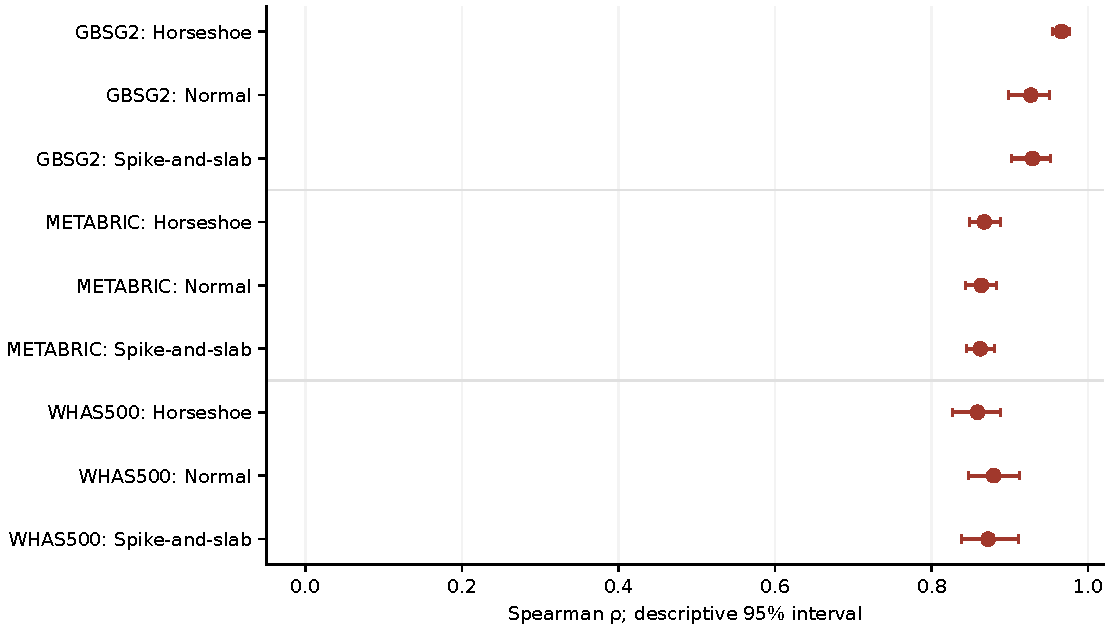
\includegraphics[width=\linewidth,height=0.7\textheight,keepaspectratio]{generated/figure_explanation_agreement.pdf}
\caption[Posterior-contribution and SHAP agreement.]{Agreement between grouped posterior contributions and same-model linear SHAP at the largest explanation budget. Intervals describe hierarchical resampling across the evaluated fits and explanation samples.}
\label{fig:explanation-agreement}
\end{figure}

\subsection{Sensitivity to Explanation Sampling}
Agreement between targets and sensitivity to sampling were assessed separately. Validation/background budgets were 25/50, 50/100 and 100/200, capped at available fold sizes, with three seeds. Stability required Spearman correlation of at least 0.95 and at least four common top-five groups in each specified comparison.

% Generated from hash-verified saved evidence. Do not edit by hand.
\begin{table}[htbp]
\centering
\caption{Explanation sampling-stability assessment.}
\label{tab:gen-explanation-gate}
\small
\setlength{\tabcolsep}{3pt}
\begin{adjustbox}{max width=\textwidth}
\begin{tabular}{rrrrl}
\toprule
\shortstack[l]{Comparison\\records} & \shortstack[l]{Evaluable\\checks} & \shortstack[l]{Within\\tolerance} & \shortstack[l]{Outside\\tolerance} & \shortstack[l]{Global stability\\criterion} \\
\midrule
1845 & 1640 & 1538 & 102 & Not satisfied \\
\bottomrule
\end{tabular}
\end{adjustbox}
\par\smallskip
\begin{minipage}{\textwidth}\footnotesize Stability was assessed across explanation budgets and seeds. The global criterion requires all evaluable checks to satisfy the specified tolerance; 102 checks were outside tolerance.\end{minipage}
\end{table}


The analysis produced \ExplanationRecords{} comparison records and \ExplanationEvaluable{} evaluable stability checks. Of these, \ExplanationPassed{} (93.8\%) met both thresholds and \ExplanationFailed{} did not. The rule requiring every evaluable check to pass was therefore not met. This result identifies sensitivity to the choice of explanation subjects, background sample and seed, even when the two explanation targets agree positively at the largest budget.

The secondary CoxPH comparison used the same subjects, background samples and seeds. For GBSG2 horseshoe, same-model agreement exceeded agreement with CoxPH by +0.156, with a descriptive 95\% interval of [+0.068, +0.256]; METABRIC horseshoe gave -0.042 [-0.060, -0.026]. The remaining intervals included zero. These paired differences describe the explanation targets within the contributing fits. Under H3a and H3b, a general stable-agreement conclusion additionally requires the sampling criteria above. Appendix~\ref{app:explainability} gives the complete paired estimates.

\section{Information-Regime and Design Robustness}
\label{sec:sensitivity-results}
\subsection{Analyses and Paired Coverage}
The robustness analyses varied training information, administrative follow-up, predictors, missing-data handling, baseline-hazard intervals and prior scales. They comprised \RobustnessPlanned{} model--condition outcomes, of which \RobustnessComplete{} met the diagnostic criteria and \RobustnessFailed{} did not. Normal and continuous spike-and-slab completed every robustness outcome; diagnostic variation occurred in the horseshoe arm.

% Generated from hash-verified saved evidence. Do not edit by hand.
\begin{table}[htbp]
\centering
\caption{Availability of paired robustness estimates.}
\label{tab:gen-robustness-coverage}
\small
\setlength{\tabcolsep}{3pt}
\begin{adjustbox}{max width=\textwidth}
\begin{tabular}{lrrrr}
\toprule
Effect family & Contrasts & Full pairs & Partial pairs & Unavailable \\
\midrule
Within-condition IBS differences & 129 & 95 & 26 & 8 \\
Difference-in-differences & 45 & 33 & 12 & 0 \\
\bottomrule
\end{tabular}
\end{adjustbox}
\par\smallskip
\begin{minipage}{\textwidth}\footnotesize The 825-condition analysis contains 770 accepted fits. Complete coverage is ten outer pairs for training-information and censoring analyses and five for design and feature sensitivities. Intervals use a hierarchical bootstrap; the tables retain each comparison\textquotesingle s paired-fold count.\end{minipage}
\end{table}


There were 129 direct prior-effect rows: 95 had full pairing, 26 partial pairing and eight no accepted estimate. Of 45 difference-in-differences, 33 had full pairing and 12 partial pairing. Intervals in this section are descriptive bootstrap intervals, with pair counts shown beside their estimates. Complete condition-level results appear in Appendix~\ref{app:sensitivity}.

\subsection{Reduced Training Information}
A difference-in-differences measures the change in IBS(Normal) minus IBS(shrinkage prior), relative to full training with observed follow-up. Positive values indicate a greater relative benefit for the shrinkage prior. Table~\ref{tab:report-information} applies one display rule to all cohorts: both shrinkage priors at the smallest training fraction and earliest administrative cut-off.

\begin{table}[p]
\centering
\footnotesize
\setlength{\tabcolsep}{3pt}
\caption{Change in the prior IBS contrast under the largest declared perturbations.}
\label{tab:report-information}
\begin{tabular}{@{}lllrr@{}}
\toprule
Cohort & Condition & Prior $B$ & Pairs & \shortstack[r]{Difference-in-differences\\95\% interval}\\
\midrule
GBSG2 & 25\% training & Horseshoe & 3/10 & -0.002549 [-0.009887, +0.003348]\\
GBSG2 & 25\% training & Spike-and-slab & 10/10 & -0.000173 [-0.000456, +0.000087]\\
GBSG2 & Median truncation & Horseshoe & 2/10 & -0.000248 [-0.001702, +0.001272]\\
GBSG2 & Median truncation & Spike-and-slab & 10/10 & -0.000022 [-0.000103, +0.000048]\\
WHAS500 & 25\% training & Horseshoe & 10/10 & +0.006323 [+0.002512, +0.010561]\\
WHAS500 & 25\% training & Spike-and-slab & 10/10 & +0.000087 [-0.000343, +0.000511]\\
WHAS500 & Median truncation & Horseshoe & 10/10 & +0.000156 [-0.000740, +0.001150]\\
WHAS500 & Median truncation & Spike-and-slab & 10/10 & -0.000008 [-0.000172, +0.000138]\\
METABRIC & 25\% training & Horseshoe & 10/10 & +0.000211 [-0.001149, +0.001508]\\
METABRIC & 25\% training & Spike-and-slab & 10/10 & +0.000031 [-0.000107, +0.000158]\\
METABRIC & Median truncation & Horseshoe & 10/10 & +0.000349 [+0.000002, +0.000734]\\
METABRIC & Median truncation & Spike-and-slab & 10/10 & -0.000013 [-0.000080, +0.000044]\\
\bottomrule
\end{tabular}
\par\smallskip
\begin{minipage}{\textwidth}\footnotesize Effects are changes in IBS(Normal) minus IBS($B$), relative to full training with observed follow-up. Positive values favour $B$ relatively more. Both shrinkage priors are shown in every cohort at 25\% training and the median administrative cut-off. Cut-offs use outer-training follow-up, including event and censored records. Intervals use the hierarchical bootstrap; paired counts show coverage.\end{minipage}
\end{table}


At 25\% training, the WHAS500 Normal minus horseshoe contrast increased by +0.006323, with a 95\% interval of [+0.002512, +0.010561] and all ten pairs. This is the clearest information-regime effect in the selected comparison. METABRIC gave +0.000211 [-0.001149, +0.001508], also with ten pairs. GBSG2 gave -0.002549 [-0.009887, +0.003348], using three of ten accepted pairs.

Continuous spike-and-slab showed smaller changes under the same training reduction: -0.000173 in GBSG2, +0.000031 in METABRIC and +0.000087 in WHAS500. Each used ten pairs and had an interval spanning zero. The results therefore identify a specific horseshoe response in WHAS500, rather than the same response for both shrinkage priors or all cohorts.

\subsection{Administrative Follow-Up}
Truncating follow-up at the median outer-training follow-up increased the Normal minus horseshoe contrast in METABRIC by +0.000349 [+0.000002, +0.000734], with ten pairs. WHAS500 gave +0.000156 [-0.000740, +0.001150]. GBSG2 supplied two accepted pairs, with a change of -0.000248 [-0.001702, +0.001272]. Continuous spike-and-slab changes were close to zero in all three cohorts.

The truncation times use all outer-training follow-up records, including censored observations. They therefore represent an administrative restriction of follow-up, while prediction horizons are defined from training-event times. Figure~\ref{fig:robustness-did} shows the full set of training-fraction and truncation contrasts, keeping these two information changes separate.

\begin{figure}[tbp]
\centering
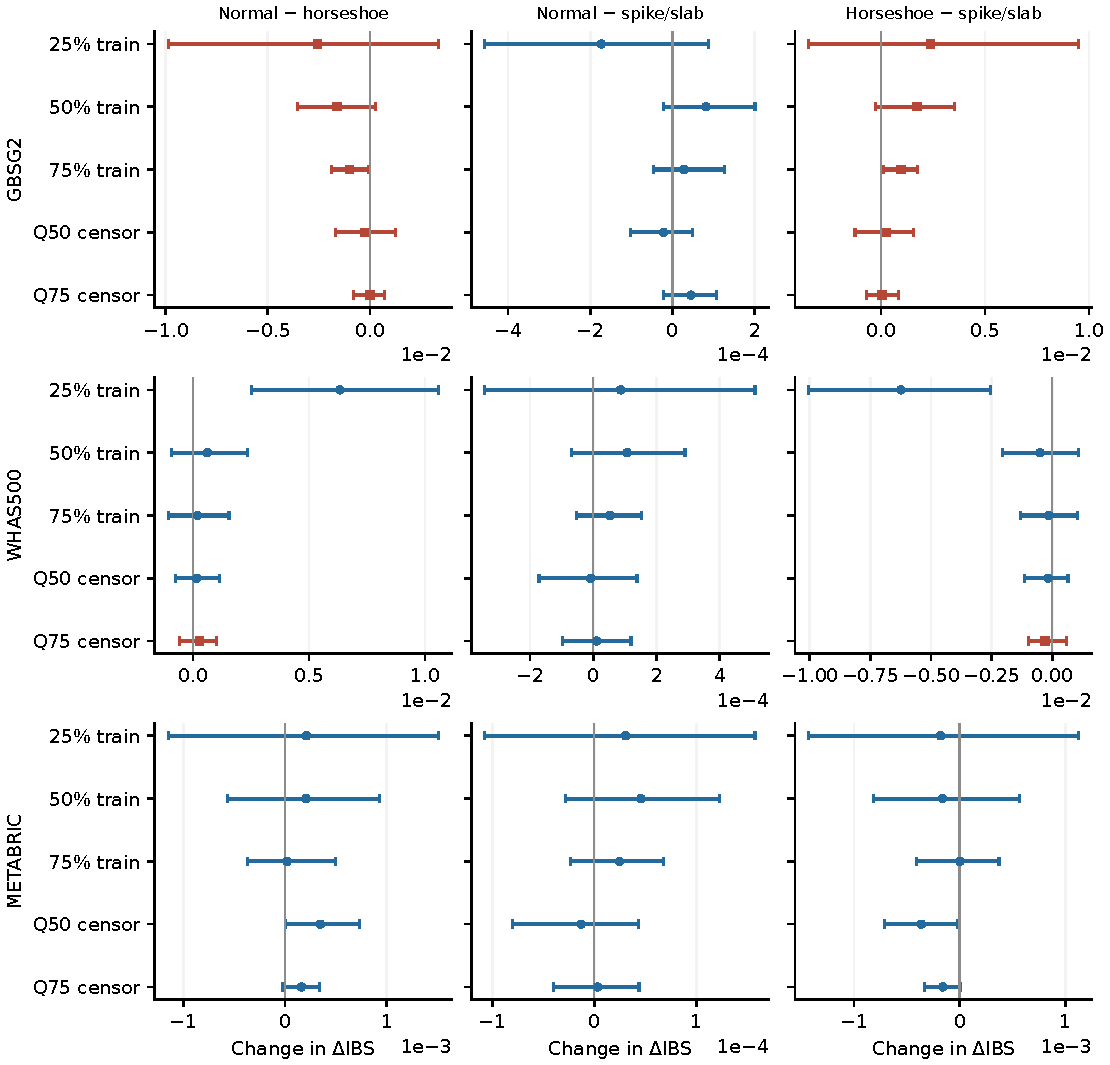
\includegraphics[width=\linewidth,height=0.75\textheight,keepaspectratio]{generated/figure_robustness_did.pdf}
\caption[Prior contrasts under changes in training information.]{Changes in the prior IBS contrast under reduced training fractions and administrative follow-up. Intervals are descriptive bootstrap intervals, and pairing counts identify the accepted evaluations contributing to each estimate.}
\label{fig:robustness-did}
\end{figure}

\subsection{Predictors, Missingness and Model Specification}
Changing baseline intervals and prior scales generally retained small Normal minus continuous-spike-and-slab differences. In GBSG2, the direct contrast was +0.000086 with four intervals and +0.000107 with ten. Under the primary, tighter and wider prior settings, it was +0.000107, +0.000041 and +0.000012. Each used all five pairs. The ten-interval interval was [+0.000009, +0.000209], while the tighter and wider prior intervals spanned zero. These analyses use outer fold 1 in each of five repeats, making their evaluation design explicit alongside the original 25-pair results.

METABRIC's Normal minus continuous-spike-and-slab contrast was +0.000017 with the Nottingham Prognostic Index components, -0.000003 after adding stage and -0.000038 with stage-inclusive multiple-imputation prediction averaging. Each had five pairs and an interval spanning zero. The multiple-imputation interval was [-0.000464, +0.000380], wider than the other two. The contrast therefore stayed close to zero across these representations, while its precision changed with the missing-data procedure.

The five-imputation analysis averaged model predictions across imputations. WHAS500's published-feature analysis included length of stay, and METABRIC's treatment-augmented analysis used treatment information. These conditions extend the predictor information available to the corresponding models; the primary specifications retain their stated clinical prediction setting. Their estimates are reported together in Appendix~\ref{app:sensitivity}.

The training-fit proportional-hazards checks repeatedly identified departures for METABRIC age and Nottingham Prognostic Index under within-fit Holm adjustment. This helps interpret the relationship between coefficient associations, calibration and predictive discrimination under the shared proportional-hazards structure. The rejection frequencies describe overlapping training samples. Appendix~\ref{app:baselines} gives the predictor-level summaries.

\section{Computational Reliability and Sampler Sensitivity}
\label{sec:diagnostic-results}
The original Bayesian evaluation accepted \BayesianComplete{} of \BayesianPlanned{} model--fold outcomes. Four-chain sampling used the criteria in Chapter~\ref{chap:methods}, including rank-normalised $\widehat R$, effective sample size, BFMI, divergences and tree-depth checks. Table~\ref{tab:gen-diagnostics} summarises the recorded diagnostic results.

% Generated from hash-verified saved evidence. Do not edit by hand.
\begin{table}[htbp]
\centering
\caption{Diagnostic acceptance and computation time by model.}
\label{tab:gen-diagnostics}
\small
\setlength{\tabcolsep}{3pt}
\begin{adjustbox}{max width=\textwidth}
\begin{tabular}{llrrr}
\toprule
Cohort & Model & Accepted & Other outcomes & Median seconds \\
\midrule
GBSG2 & CoxPH & 25 & 0 & 3.9 \\
GBSG2 & RSF & 25 & 0 & 11.9 \\
GBSG2 & DeepSurv & 25 & 0 & 5.8 \\
GBSG2 & Normal & 25 & 0 & 17.8 \\
GBSG2 & Horseshoe & 7 & 18 & 399.5 \\
GBSG2 & Spike-and-slab & 25 & 0 & 58.3 \\
WHAS500 & CoxPH & 25 & 0 & 3.4 \\
WHAS500 & RSF & 25 & 0 & 8.9 \\
WHAS500 & DeepSurv & 25 & 0 & 4.9 \\
WHAS500 & Normal & 25 & 0 & 20.9 \\
WHAS500 & Horseshoe & 25 & 0 & 131.2 \\
WHAS500 & Spike-and-slab & 25 & 0 & 60.8 \\
METABRIC & CoxPH & 25 & 0 & 6.4 \\
METABRIC & RSF & 25 & 0 & 56.7 \\
METABRIC & DeepSurv & 25 & 0 & 10.0 \\
METABRIC & Normal & 25 & 0 & 103.8 \\
METABRIC & Horseshoe & 23 & 2 & 683.8 \\
METABRIC & Spike-and-slab & 25 & 0 & 355.0 \\
\bottomrule
\end{tabular}
\end{adjustbox}
\par\smallskip
\begin{minipage}{\textwidth}\footnotesize Each cohort--model combination contains 25 outer evaluations. Median computation time includes the specified fitting attempts.\end{minipage}
\end{table}


Normal and continuous spike-and-slab each supplied all 75 Bayesian evaluations across the three cohorts. Horseshoe supplied 55 of 75: seven in GBSG2, 25 in WHAS500 and 23 in METABRIC. The 18 GBSG2 and two METABRIC diagnostic outcomes account for the four primary contrasts without complete pairing. Thus computational reliability contributes directly to the scope and precision of the prior comparison.

The specified remedies increased warm-up and, in the second remedy, used a non-centred baseline-hazard parameterisation while retaining the likelihood and prior. The separate higher-target-acceptance analysis examines a further computational change on the same original folds.

\subsection{Post-Hoc Higher-Target-Acceptance Analysis}
\label{sec:posthoc-results}
The post-hoc horseshoe analysis used target acceptance 0.999 on every original outer fold. All \SensitivityComplete{} of \SensitivityPlanned{} horseshoe evaluations met the diagnostic criteria. Table~\ref{tab:gen-sampler-sensitivity} compares their predictions with the unchanged Normal and continuous spike-and-slab predictions.

% Generated from hash-verified saved evidence. Do not edit by hand.
\begin{table}[htbp]
\centering
\caption{Post-hoc sampler sensitivity with target acceptance 0.999.}
\label{tab:gen-sampler-sensitivity}
\small
\setlength{\tabcolsep}{3pt}
\begin{adjustbox}{max width=\textwidth}
\begin{tabular}{llrrrr}
\toprule
Cohort & Contrast ($A-B$) & Pairs & $\Delta$IBS & Nominal 95\% interval & $p_{\mathrm{Holm}}$ \\
\midrule
GBSG2 & Normal - Horseshoe & 25 & -0.000081 & [-0.001780, +0.001618] & 1.000 \\
GBSG2 & Normal - Spike-and-slab & 25 & +0.000025 & [-0.000103, +0.000153] & 1.000 \\
GBSG2 & Horseshoe - Spike-and-slab & 25 & +0.000106 & [-0.001476, +0.001688] & 1.000 \\
WHAS500 & Normal - Horseshoe & 25 & +0.000346 & [-0.001689, +0.002382] & 1.000 \\
WHAS500 & Normal - Spike-and-slab & 25 & +0.000061 & [-0.000120, +0.000242] & 1.000 \\
WHAS500 & Horseshoe - Spike-and-slab & 25 & -0.000286 & [-0.002161, +0.001590] & 1.000 \\
METABRIC & Normal - Horseshoe & 25 & -0.000486 & [-0.001581, +0.000609] & 1.000 \\
METABRIC & Normal - Spike-and-slab & 25 & -0.000008 & [-0.000087, +0.000071] & 1.000 \\
METABRIC & Horseshoe - Spike-and-slab & 25 & +0.000478 & [-0.000559, +0.001514] & 1.000 \\
\bottomrule
\end{tabular}
\end{adjustbox}
\par\smallskip
\begin{minipage}{\textwidth}\footnotesize This post-hoc sensitivity contains 75 accepted horseshoe fits at target acceptance 0.999, paired with the original Normal and continuous spike-and-slab predictions. Original and sensitivity results retain separate identities.\end{minipage}
\end{table}


All nine contrasts had 25 pairs. Normal minus horseshoe was -0.000081 in GBSG2, +0.000346 in WHAS500 and -0.000486 in METABRIC. Every nominal repeated-validation interval included zero, and every Holm-adjusted $p$ value was one. The analysis adds complete diagnostic acceptance under the higher target while retaining the small predictive differences observed between the tested priors. These post-hoc estimates are reported separately from the original sampling configuration.

\subsection{Post-Hoc Bound for the Primary Holm Family}
The nine-comparison original family contains five observed tests and four unavailable tests. A post-hoc sensitivity calculation bounded the Holm-adjusted values of the observed tests by setting the four missing $p$ values to their extremes. The best and worst bounds were one for each observed test. Consequently, none of the five observed tests is rejected at 0.05 for any completion of the missing values. Table~\ref{tab:gen-holm-bounds} in Appendix~\ref{app:sampler} gives the bounds. This calculation concerns the five observed tests; it does not impute the other four effects.

\section{Integrated Discussion}
\subsection{Prior Choice as a Joint Prediction and Computation Question}
The controlled likelihood and shared validation make the prior comparison particularly clear. Normal and continuous spike-and-slab gave closely aligned IBS in all three cohorts. Horseshoe supplied a similar complete-fold predictive picture in WHAS500, while its original diagnostic acceptance varied across cohorts. The higher-target-acceptance analysis then achieved complete acceptance with small predictive changes. Together, these findings show how prior choice can affect computation even when its measured effect on probability prediction is modest.

The controlled information reductions provide a more specific view of shrinkage behaviour than comparing unrelated cohort sizes. In WHAS500, the horseshoe contrast shifted in its favour at 25\% training. METABRIC showed a smaller change, and continuous spike-and-slab stayed close to its full-information contrast in all three cohorts. These results locate the observed information effect within a particular prior, clinical setting and evaluation condition.

\subsection{Discrimination, Probability Error and Calibration}
The METABRIC comparator results demonstrate the value of examining model families alongside coefficient priors. RSF had both lower IBS and higher discrimination than the linear models, and the paired IBS interval against Normal favoured the forest. WHAS500 showed a different ordering, with the complete Bayesian arms and CoxPH providing the lower mean IBS values. This pattern is consistent with comparative survival research that evaluates methods across several datasets rather than assuming a common hierarchy \cite{ravi33,ravi37,ravi73,ravi79}.

Calibration adds information beyond that ordering. Near-zero fixed-slope offsets coexisted with slopes different from one, particularly in GBSG2. Conversely, similar IBS values for Normal and continuous spike-and-slab coincided with similar calibration summaries. Reporting these quantities together gives a more complete account of the probability predictions than any individual metric.

\subsection{Posterior Interpretation and Explanation Sampling}
Posterior coefficients, transformed hazard ratios and directional probabilities express associations and their uncertainty on a defined predictor scale. Grouped contributions add a common importance target across priors. Their positive agreement with same-model SHAP shows that these summaries often identify similar leading predictor groups.

The stability experiment asks a further question: how much those rankings change when the explanation sample changes. Its 93.8\% threshold pass rate and unmet all-comparisons criterion distinguish broad descriptive agreement from uniform sampling stability. The combination of posterior interpretation, target agreement and sampling assessment makes these different properties visible within one empirical analysis.

\section{Research Question Synthesis}
Table~\ref{tab:research-answers} links the research questions and hypotheses to their empirical findings.

\begin{table}[htbp]
\centering
\singlespacing
\small
\caption{Research questions and empirical findings.}
\label{tab:research-answers}
\begin{tabularx}{\textwidth}{@{}>{\raggedright\arraybackslash}p{0.17\textwidth}>{\raggedright\arraybackslash}X>{\raggedright\arraybackslash}p{0.29\textwidth}@{}}
\toprule
Question & Main evidence & Interpretation\\
\midrule
RQ1; H1: coefficient priors and event information & Normal minus continuous spike-and-slab IBS ranges from -0.000008 to +0.000061. All five complete original prior intervals include zero. & Prior effects are small within these clinical predictor sets. The complete original contrasts do not identify a general predictive advantage associated with lower event information.\\[0.5em]
RQ2; H2: reduced training information & At 25\% training, the horseshoe contrast changes by +0.006323 in WHAS500 and +0.000211 in METABRIC, each with ten pairs. & The relative shrinkage benefit changes by prior and cohort, with the clearest observed effect in WHAS500 horseshoe.\\[0.5em]
RQ3; H3a: same-model explanation agreement & Spearman agreement ranges from 0.859 to 0.966. Of 1,640 evaluable stability checks, 1,538 meet both thresholds. & Positive target agreement accompanies sensitivity to explanation sampling; the all-comparisons stability criterion is not met.\\[0.5em]
RQ3; H3b: paired comparison with CoxPH & Same-model-minus-CoxPH agreement varies in direction across cohort--prior combinations. & These are descriptive paired estimates. The required stability condition for a general stronger-agreement conclusion is not met.\\[0.5em]
RQ4: predictor and model specification & Training, follow-up, feature, imputation, interval and prior-scale conditions give small but variable effects with reported pairing. & Robustness is described at the level of the specified condition, predictor information and accepted evaluations.\\
\bottomrule
\end{tabularx}
\end{table}
